\chapter{UEFI BIOS自动化测试工具SCT的设计与实现}
\label{cha:intro}
	
	UEFI BIOS作为新一代的BIOS,在其开发过程中,需要开发人员对源文件频繁地进行重构,这就需要对其的测试工作是可以自动化、简洁、高速运行的,否则代码的重构也就是不现实的。与传统的软件测试工作相比而言,UEFI BIOS的软件测试工作与之有着很多的不同点:UEFI BIOS软件的运行并不是在OS(Operating System:操作系统)环境中,而是在计算机加载操作系统之前运行,而现有的测试工具均是运行在操作系统环境之中的,因而现有的测试工具均无法正常运行在UEFI BIOS环境中,在被测机器上对其进行测试。而利用测试工具对已构建、部署好的产品进行验证和测试同样也是UEFI BIOS持续集成测试系统的基础。 因此,设计一套拥有良好性能和稳定可靠的测试工具用于UEFI BIOS的测试就成为了我们首先要解决的问题。
	
\section{自动化测试工具的设计目标}

	在基于EFI$\backslash$UEFI标准下,我们需要结合UEFI BIOS中测试的实际需求,开发一套自动化测试工具SCT用于测试UEFI BIOS中各种类库的正确性和有效性。SCT能够在UEFI BIOS的Shell环境中运行,对产品进行白盒、黑盒等不同类型的测试,自动化的执行用例以对产品进行验证,并且能够以测试报告的形式作为结果,便于QA对测试整体进行查看。
	
\section{ 自动化测试工具的需求分析}

  该测试工具需要具有以下特点:

  \begin{itemize}
    \item 能够自动化的执行用例,对UEFI BIOS进行测试和验证,及时发现其中可能存在的问题和缺陷,以便于提高软件的质量。
	\item 需要能够执行多种类型的测试任务,例如白盒、黑盒等不同类型的测试。
	\item 能够分析每一个用例的测试结果和日志,对全部用例进行总结,生成相应的测试报告。
	\item 具备完善的日志功能,便于QA查看测试工具的运行记录。
	\item 当工具运行发生意外中断时,能够记录中断的位置,在工具再次执行时从该位置继续执行之后的用例。
	\item 需要具备良好的GUI,方便QA能够便捷的对测试工具进行设置,控制需要执行的用例。
	\item 由于良好的扩展性是产品的一个特点,因此工具应该具备方便添加相应的测试库这一重要的功能属性。
  \end{itemize}

\section{自动化测试工具的系统功能组成分析}

	根据对SCT的需求进行分析和归纳,本文进一步对其系统的各个组成功能进行了设计,得出最终的UEFI BIOS测试工具SCT的系统功能组成框架如图~\ref{fig:自动化测试工具的功能组成框架图}所示:
	
	\begin{figure}[H] % use float package if you want it here
		\centering
		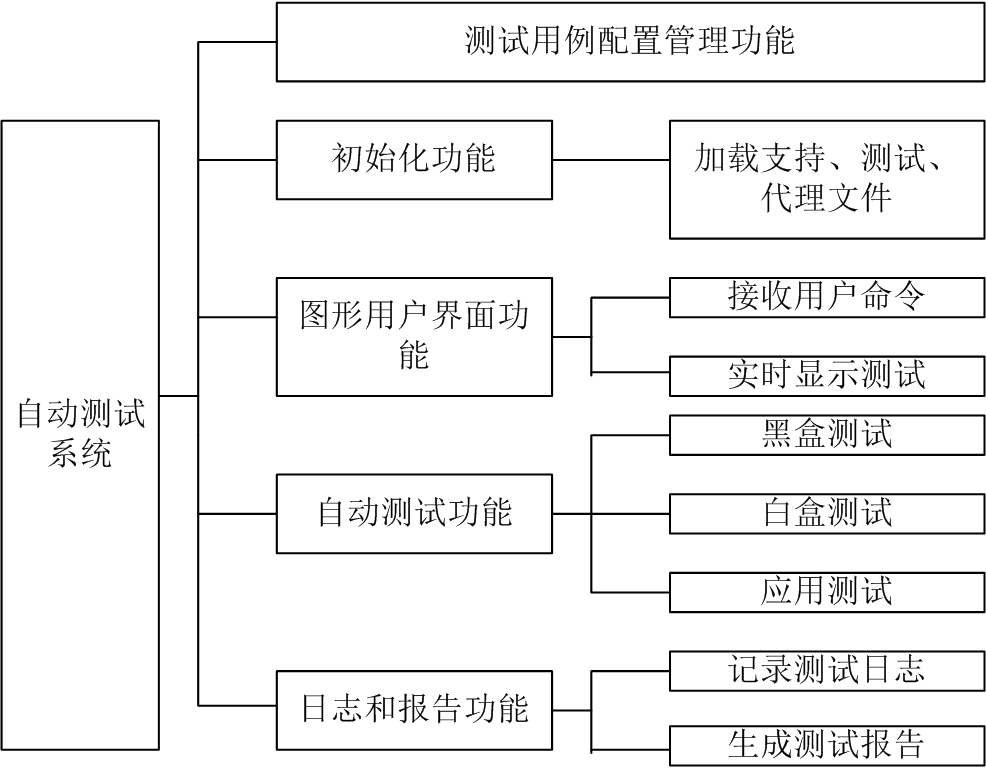
\includegraphics[height=8cm]{chart3/自动化测试工具的功能组成框架图}
		\caption{自动化测试工具的功能组成框架图}
		\label{fig:自动化测试工具的功能组成框架图}
	\end{figure}
	
	\begin{itemize}
		\item 用例配置管理的功能
		
		SCT需要在运行并对产品进行测试之前首先进行配置,主要是通过加载配置文件的方法来实现该功能。将对一切用例文件的描述信息存入到一个配置文件里,测试工具启动运行时对其进行读取并且使用。
		\item 初始化的功能
		
		在工具启动时自动加载测试、代理和支持文件,而这些文件也正是工具所必须的文件,这一功能即为初始化功能。所加载的各种文件是提前通过编译构建好的可执行文件,这些文件的后缀为.efi。测试工具SCT在运行测试任务时,每一个测试文件都有相对应的代理文件与之匹配,通过代理文件其读取所需要测试功能函数的相关信息,以便于验证该函数的正确性。
		\item 图形用户界面的功能
		
		GUI用于展示工具中的用例及策略,按照QA的思路便于QA对策略进行修改,并且能够实时的将测试的相关信息在测试前、中、后展示给QA,在测试后将每一个Case的执行情况以及执行结果通过GUI展示给相关的QA。
		\item 自动化测试的功能
		
		SCT的核心功能部分便是自动化测试功能,它按照QA的意愿对其所需执行的用例自动化的执行。工具运行对测试文件进行加载,操纵测试的进度,自动化的寻找并且执行下一个用例。当出现中断问题时,工具会对此次的中断点进行储存,工具再次运行时会首先提示QA是否在断点的基础上执行之后未完成的部分,这大大提高了测试的可持续性。
		\item 日志和生成报告的功能
		
		SCT能够将对每个Case的执行情况和结果进行记录,并且根据这些记录QA能够利用SCT自动化的生成该轮测试任务的报告,这就是日志和生成报告的功能。这一功能便于QA从整体上来观察和判断此轮测试任务的进展和结果。SCT将每一个Case的运行情况和结果自动记录到其对应的每一个日志文件当中,利用这一些日志文件,SCT能够自动化的生成CSV报告,它能够对所有的用例的执行结果进行概括。
	\end{itemize}
	
\section{自动化测试工具的系统功能流程分析}
	
	QA首先将用例和代理文件放在测试工具相应的目录下,SCT运行时首先进行初始化,通过配置文件的管理加载所需要的用例,将所需要的文件载入到测试工具中,并且提取出文件中包含的测试单元和用例,进入图形化用户操作界面。之后QA通过GUI选择、配置、执行用例,SCT就自动化的运行已选的用例,进行白盒、黑盒测试,同时生成相关的日志。任务完成后QA通过SCT提供的功能能够自动化的生成初步的报告。
	
	综上所述,可以得出UEFI BIOS测试工具SCT的系统功能流程如图~\ref{fig:自动化测试工具的功能流程图}所示:
	
	\begin{figure}[H] % use float package if you want it here
		\centering
		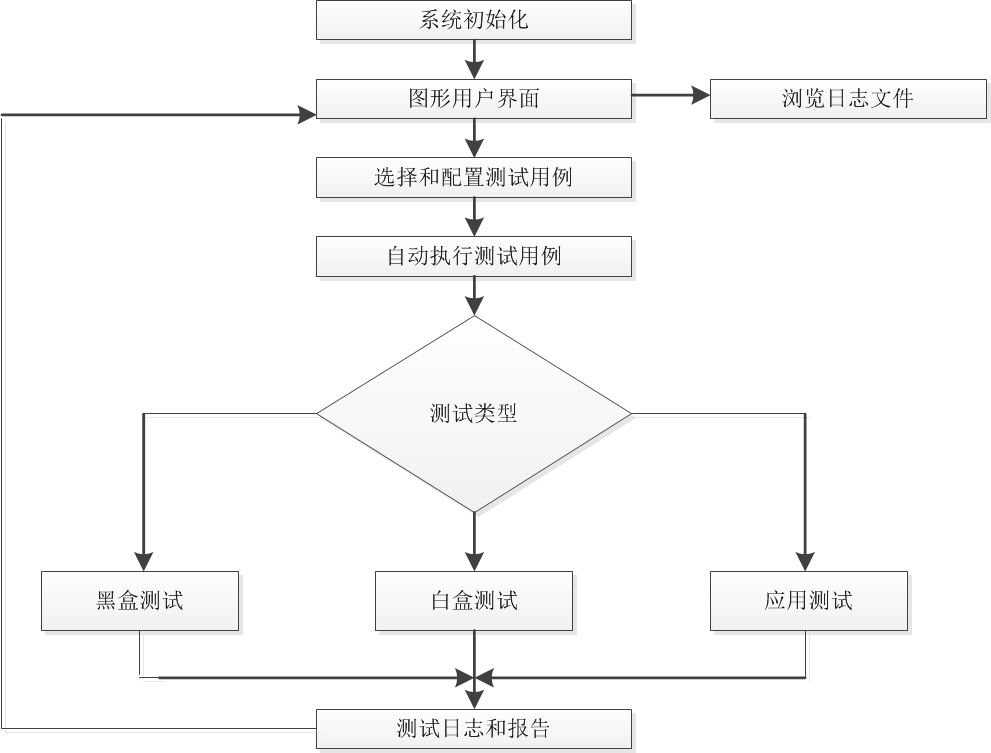
\includegraphics[height=10cm]{chart3/自动化测试工具的功能流程图}
		\caption{自动化测试工具的功能流程图}
		\label{fig:自动化测试工具的功能流程图}
	\end{figure}
	
\section{自动化测试工具的设计方案}
	
	在分析了测试工具的功能组成架构和功能流程的基础上,本小节将对该系统主要功能的设计和实现进行描述。
	
	\subsection{自动化测试工具中储存结构的设计及文件的载入}
		
		SCT储存的结构分为外部和内部两部分,外部的储存由配置文件和日志文件两部分组成,内部的储存则是文件以及Case在SCT内部结构的描述,这一小节我们主要对其进行讨论。
		
		\begin{itemize}
			\item 测试函数库以及测试用例管理配置的详细设计
				\begin{itemize}
					\item 测试库配置管理
					
					在工具启动并初始化以及在用例执行时,我们需要寻找合适的方法向用户提供一些被测试函数库的描述信息供其使用。考虑到被测试函数库的信息在项目开发的进行中是基本不会被修改的,因此我们创建一个文件夹,利用配置文件来存储所有的被测试函数库的基本信息,供测试工具加载使用。
						
					针对配置文件中的信息格式,我们设计了五个属性用于对被测试函数库进行描述,主要由Revision、CategoryGuid、InterfaceGuid、Name和Description构成。其中Revision代表被测试函数库的产品版本号,所有被测试函数库的版本号通常情况下都是0x00010000;CategoryGuid代表该被测试函数库的唯一标识;InterfaceGuid代表该被测试函数库的一个实例的GUID,其中GUID是UEFI BIOS开发中针对每个函数库以及其实例所设定的一个唯一的标识;Name代表被测试函数库的名称;Description代表被测试函数库的描述信息。以GenericTest为例它的配置信息如图~\ref{fig:测试库配置管理中配置信息的设计}所示:
						\begin{figure}[H] % use float package if you want it here
							\centering
							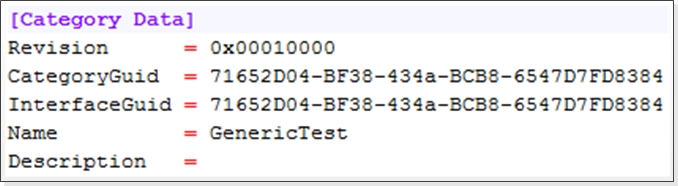
\includegraphics[height=3cm]{chart3/测试库配置管理中配置信息的设计}
							\caption{测试库配置管理中配置信息的设计}
							\label{fig:测试库配置管理中配置信息的设计}
						\end{figure}
							
					.ini文件为UEFI BIOS所规定的配置文件格式,所以设计的配置文件,其命名为Category.ini,其中包含了所有被测试函数库的相关信息,SCT在启动运行时自动加载该配置文件并且读取其中的内容,从而获取所有被测试函数的描述信息。
					
					\item 用例配置管理
					
						一个测试用例对应一个被测试函数,被测试函数库由相应的测试用例集所对应,为了存储测试用例的相关描述内容,我们创建了一个文件用于保存这些内容,这个文件叫做Seq.seq,用以在自动化测试工具中保存测试用例的信息。每一个测试用例的信息由四部分内容所组成:Revision代表测试用例的版本号,通常情况下其默认版本号为0x10000;GUID代表UEFI BIOS规定的被测试函数的唯一标识;Name代表被测试的函数,即被测试函数的名称;Order代表此用例在该轮测试的执行顺序,通常其默认值为0xFFFFFFFF,自动化测试工具会按照该配置文件中测试用例的顺序依次执行;Iterations代表该测试用例被迭代测试的次数。以GetState-Func函数为例,其对应测试用例的配置信息如图~\ref{fig:测试用例配置管理中配置信息的设计}所示:
							\begin{figure}[H] % use float package if you want it here
								\centering
								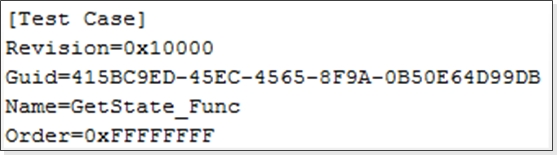
\includegraphics[height=3cm]{chart3/测试用例配置管理中配置信息的设计}
								\caption{测试用例配置管理中配置信息的设计}
								\label{fig:测试用例配置管理中配置信息的设计}
							\end{figure}
				\end{itemize}
			\item 文件结构和用例结构详细设计
			
				SCT自动化测试工具需要在启动并且运行时加载四类文件,其中包括配置文件、代理文件、支持文件以及测试文件。为了载入这四类文件,SCT在启动运行后,加载并且遍历该四类文件各自所属文件夹下的所有内容,其以整个文件目录为目标进行加载,在加载后对其进行判断,若是所需文件,则以文件为单元,载入到计算机内存中便于后续对其使用。为了支持系统例如恢复、日志和Assertion等功能,本文将这些功能通过.efi文件的形式进行实现,并且以主目录下Support文件夹的Driver文件以及Application文件等形式进行存放,SCT启动运行后便会加载这些.efi文件从而实现这一系列的功能。为了将载入工具中的剩余文件在系统中保存,我们利用结构体和链表的形式对其进行设计和实现,来保存其他的文件。
		\end{itemize}
	\subsection{自动化测试工具的各个模块设计}
		
		整个SCT由四部分功能模块共同构成:GUI图形用户操作界面、自动化测试运行、SCT初始化、日志和报告反馈这四部分模块。若干个小的功能模块构成了每一个模块部分,其整体结构组成如图~\ref{fig:自动化测试工具的纵向结构图}所示。下面是有关各个模块详细设计的讨论。
		
		\begin{figure}[H] % use float package if you want it here
			\centering
			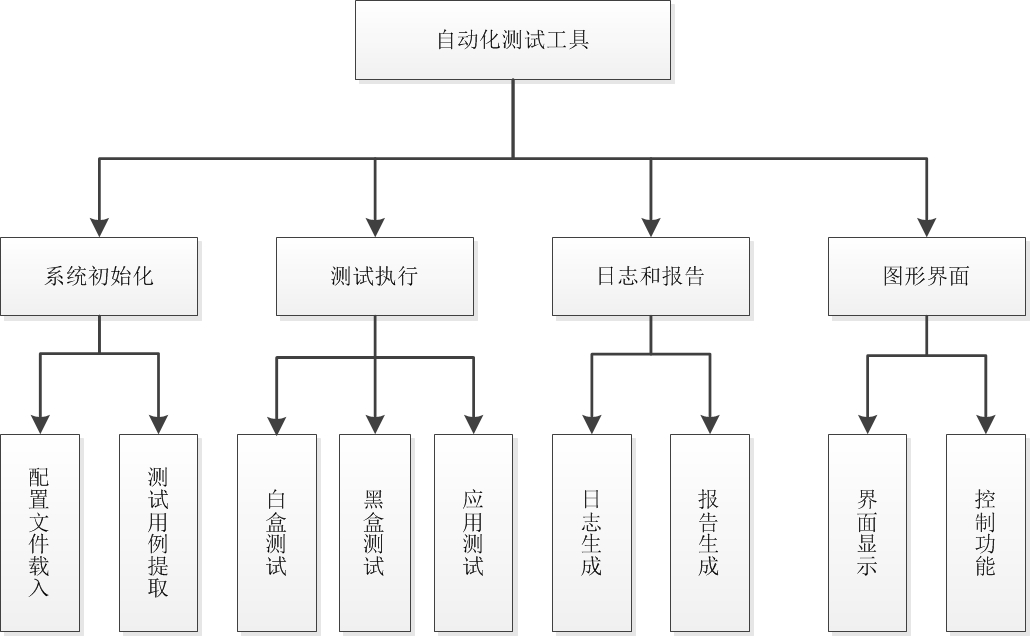
\includegraphics[height=8cm]{chart3/自动化测试工具的纵向结构图}
			\caption{自动化测试工具的纵向结构图}
			\label{fig:自动化测试工具的纵向结构图}
		\end{figure}
		
		\begin{itemize}
			\item 初始化模块详细设计
			
				该模块是对SCT启动并且初始化进行支持,它将SCT所需的文件加载,读取所有用例和初始化用例的状态。其主要分为两个部分:第一个部分为SCT载入代理、配置文件;第二个部分为SCT加载测试文件,并且从中提取Case的相关内容,从而确定该轮测试任务所要执行用例的情况,并且设定测试用例的状态。其流程如图~\ref{fig:初始化模块流程图}所示:
			
				\begin{figure}[H] % use float package if you want it here
					\centering
					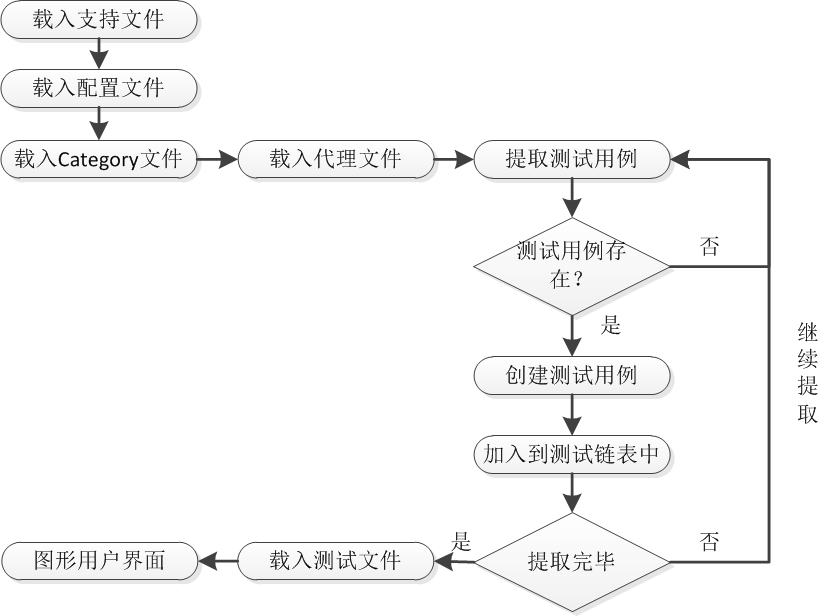
\includegraphics[height=9cm]{chart3/初始化模块流程图}
					\caption{初始化模块流程图}
					\label{fig:初始化模块流程图}
				\end{figure}
			
			\item 自动化执行模块详细设计
			
				有两种方法可以用于自动化的运行测试:第一种是通过GUI,QA利用键盘等外设选择该轮测试任务所需要执行的Case,然后选择执行,SCT便会对其自动化的执行各种类型的测试任务;第二种则是QA通过在SCT运行前修改和设置文件配置相关信息,从而通过其文件中指定的执行所需用例,这样能够通过配置文件提前将每轮测试任务所需要执行的Case提前设置好,而不需要每次通过第一种方法GUI界面操作的方法来对其进行设置。自动化执行模块的功能流程如图~\ref{fig:自动化执行模块流程图}、~\ref{fig:自动化执行模块中测试功能部分的流程设计}所示:
			
				\begin{figure}[H] % use float package if you want it here
					\centering
					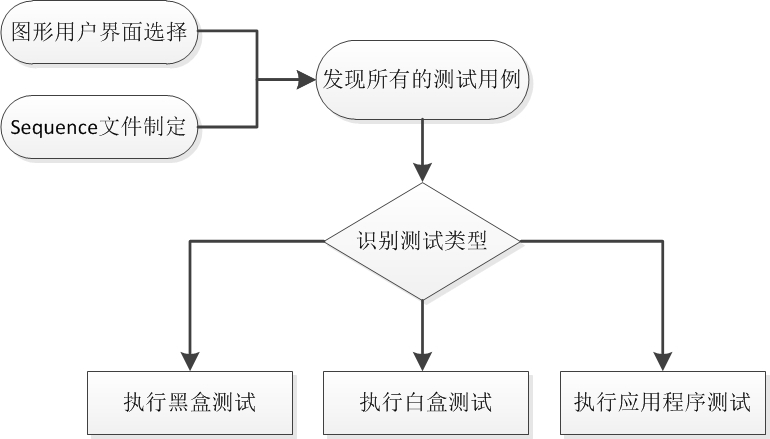
\includegraphics[height=6.5cm]{chart3/自动化执行模块流程图}
					\caption{自动化执行模块流程图}
					\label{fig:自动化执行模块流程图}
				\end{figure}
			
				\begin{figure}[H] % use float package if you want it here
					\centering
					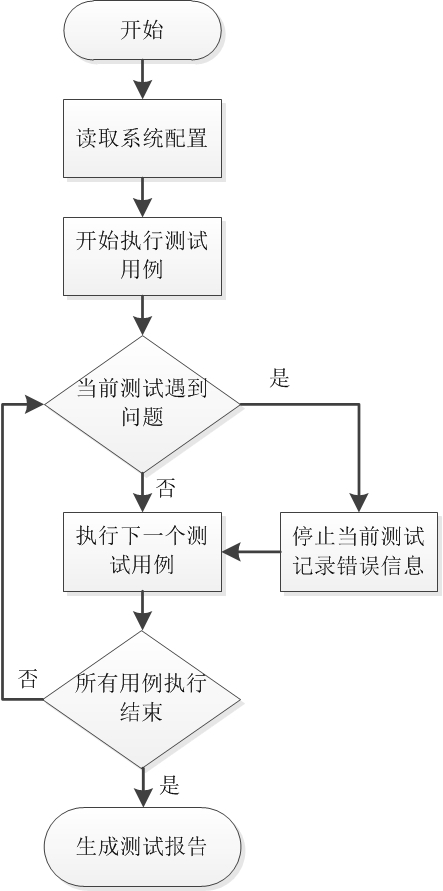
\includegraphics[height=14cm]{chart3/自动化执行模块中测试功能部分的流程设计}
					\caption{自动化执行模块中测试功能部分的流程设计}
					\label{fig:自动化执行模块中测试功能部分的流程设计}
				\end{figure}		
			
			\item 日志和报告模块详细设计
				\begin{itemize}
					\item 日志部分设计
					
						每一运行的用例由一个日志文件相对应,文件中的信息分为7个部分,如图~\ref{fig:日志文件设计图}所示:
						
						\begin{figure}[H] % use float package if you want it here
							\centering
							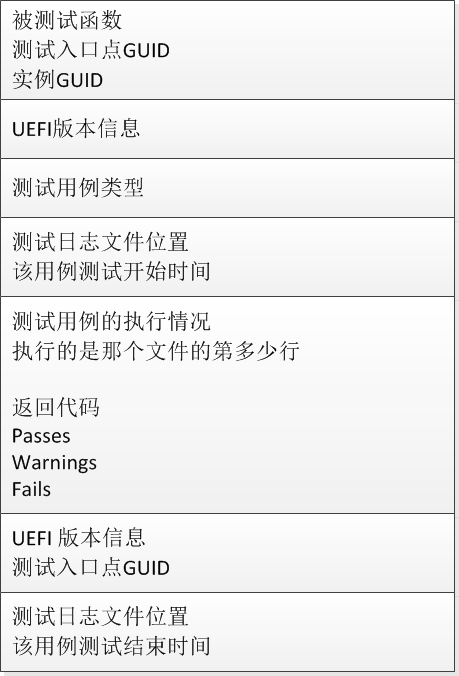
\includegraphics[height=11cm]{chart3/日志文件设计图}
							\caption{日志文件设计图}
							\label{fig:日志文件设计图}
						\end{figure}
						
						为了实现测试日志这一功能,SCT利用支持文件对其进行设计与实现。为了向SCT提供需要测试的功能,本文将测试日志部分设计成为驱动,在SCT启动并且初始化时,首先将该驱动加载到工具中。和面向对象设计中的类相似,本文将自动化测试工具中实现测试功能的部分设计为Protocol,由数据成员和相应的功能函数所构成,其名称为TLL(Test Logging Library)。TLL由构造函数TLLBeginLogging、析构函数TLLEndLogging和其他一些功能函数共同组成。TLLBeginLogging的主要功能为:加载所需被运行测试用例的相关内容,为测试日志的生成在操作系统中提前分配好所需的空间内存,创建好所需的相关结构体,并且打开日志文件对其测试执行过程中的相关信息进行记录。TLLEndLogging的主要功能为:关闭打开的日志文件,释放之前分配的内存空间。我们还设计了一个函数命名为TLLSetConfig,用于在自动化测试工具启动时对其日志模块进行设置。在设计好的日志功能中,还有一个最为重要的函数TLLWriteLogFile,他的主要功能是将测试过程中的日志信息写入到相关的日志文件中。综上所述,日志功能的设计如图~\ref{fig:日志功能的设计表}所示:
						
						\begin{figure}[H] % use float package if you want it here
							\centering
							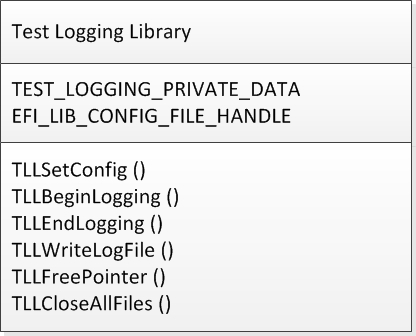
\includegraphics[height=6cm]{chart3/日志功能的设计表}
							\caption{日志功能的设计表}
							\label{fig:日志功能的设计表}
						\end{figure}	
					
					\item 报告部分设计
					
						该模块是SCT的一个重要组成功能,它以日志为基础,对此次测试验证的结果进行统计和概述,其内容主要包含用例的数量,每个用例的执行结果等相关信息,这使得QA节省了自己动手统计的时间成本。
						
						针对报告中信息的格式的设计,以测试需求为基础,将其分为两部分内容:第一部分为概述信息,说明了所测试函数的名称、用例的总个数、失败用例以及通过用例的数量;第二部分则是测试过程中的相关信息,未通过在前通过的在后。如图~\ref{fig:测试报告文件格式设计}所示:
						
						\begin{figure}[H] % use float package if you want it here
							\centering
							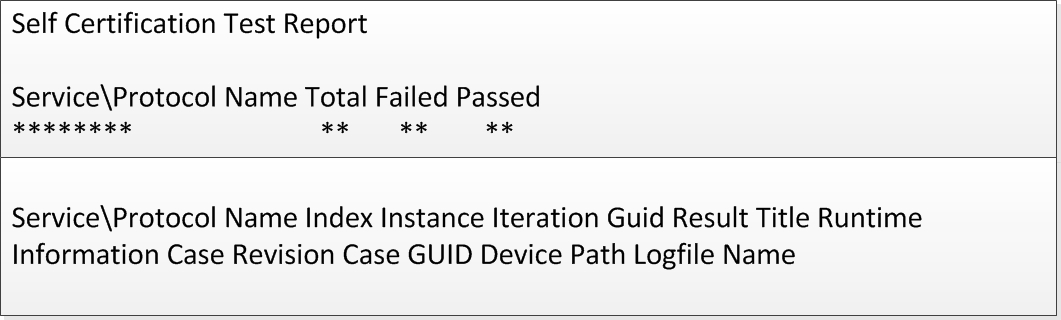
\includegraphics[height=3.7cm]{chart3/测试报告文件格式设计}
							\caption{测试报告文件格式设计}
							\label{fig:测试报告文件格式设计}
						\end{figure}	
						
						该格式的报告,不仅对本轮测试进行了概述,同时也对每一个用例进行了详细的描述,这便于QA能够对本轮测试工作每一个Case的进展进行清楚地了解。
					\item 测试报告生成流程设计
					
						测试报告的自动生成,是指SCT通过测试过程中产生的日志文件,对其中的信息进行解析和总结,从而形成测试报告文件,便于QA从整体上来把握此轮测试的结果这一重要的过程。本文设计好的该过程的流程如图~\ref{fig:测试报告生成流程图}所示:
						
						\begin{figure}[H] % use float package if you want it here
							\centering
							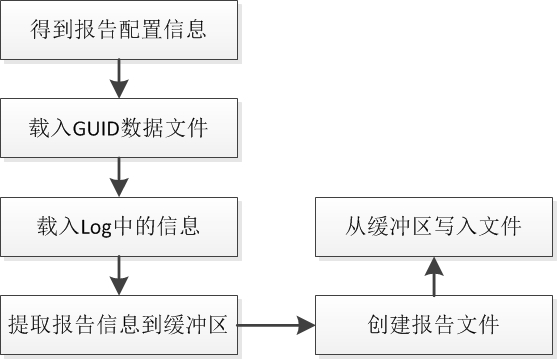
\includegraphics[height=6.5cm]{chart3/测试报告生成流程图}
							\caption{测试报告生成流程图}
							\label{fig:测试报告生成流程图}
						\end{figure}	
						
					\item 图形用户界面详细设计
					
						良好的GUI是用于QA与工具交互的接口,其是一款具有良好实用性的软件最为重要的组成之一。由于SCT运行在特定的BIOS环境之中,缺乏现有GUI库进行利用和支持,因此SCT的GUI能够尽量满足QA的需求即可。
						
						GUI主要由结构、交互和视觉设计三个部分组成:
						\begin{itemize}
							\item 结构设计
							
								SCT的GUI主要由Page、Menu、Item、Dialog四部分共同组成。相对于Web的GUI,SCT的GUI相对简便,SCT的GUI界面我们用Menu来形容,其界面上由大量的Item构成。Dialog作为对话框主要用于查看测试的文件、日志等内容。
							\item QA与SCT的交互设计
							
								该部分是通过对QA进行详尽的提示,并且利用例如键盘等外设所具备的功能对工具进行操作所组成。例如通过键盘等外设对测试工具进行操作这一功能,是通过设计和实现一个单独的.c文件,通过其来进行实现。它不仅对键盘等外设的例如上下左右空格等功能键的基本功能进行了实现,而且还设计实现了特有的快捷键功能,例如:在主界面中和用例界面点击F9,即可对所有设置好的用例运行,执行功能性测试。
							\item 视觉设计
							
								SCT的界面需要清晰明了、协调一致,能够提供撤销、恢复的功能,同样功能用同样的图形表示,色彩上应该少于等于五个色彩系列,相似的功能应该以相似的色彩来代表,少用红色以及绿色。
						\end{itemize}
				\end{itemize}
		\end{itemize}

\section{自动化测试工具的实现与使用}
	
	最终实现的UEFI BIOS自动化测试工具SCT的文件结构如图~\ref{fig:自动化测试工具SCT下的文件结构}所示:
	
	\begin{figure}[H] % use float package if you want it here
		\centering
		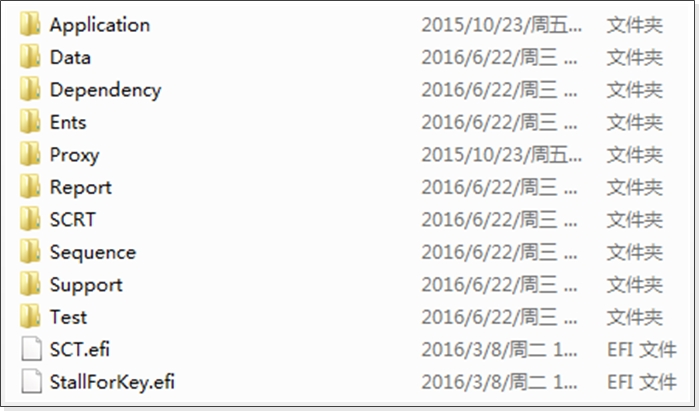
\includegraphics[height=7cm]{chart3/自动化测试工具SCT下的文件结构}
		\caption{自动化测试工具SCT下的文件结构}
		\label{fig:自动化测试工具SCT下的文件结构}
	\end{figure}
	
	\subsection{自动化测试工具的命令行控制}
	
	针对UEFI BIOS环境下对SCT的操作和控制,本文在UEFI BIOS的Shell环境下设计和实现了一个小型的命令行处理功能环境,在计算机开机但还未进入OS的情况下,用户可以通过键盘选择进入UEFI BIOS Shell命令行处理程序,在该环境下对SCT进行操作和控制。Shell是 UEFI BIOS特有的命令解析器,存在于 UEFI BIOS 中,是功能齐全的执行和调试环境用于在UEFI BIOS中进行各种设置和操作。
	
	最终实现的SCT在UEFI BIOS的Shell环境中运行。重启 PC,进入到UEFI BIOS Shell 命令行下,进入到自动化测试工具所在的目录,即可通过命令加参数运行对该工具进行操作。如图~\ref{fig:SCT-without-Parameters-Screen-Display-Using-the-Command-Line-Interface}、表~\ref{tab:自动化测试工具SCT的参数列表}所示:
	
	\begin{figure}[H] % use float package if you want it here
		\centering
		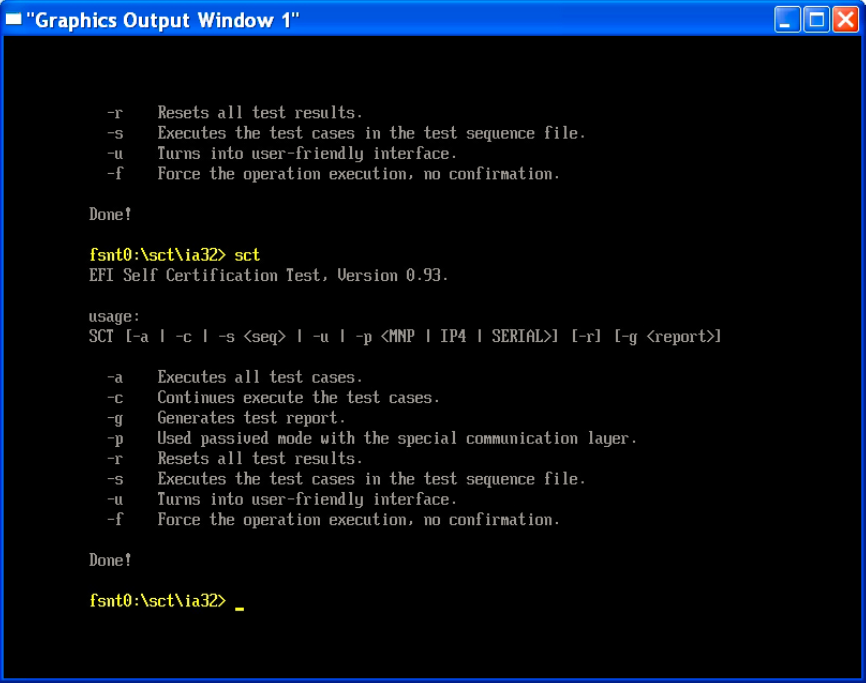
\includegraphics[height=8cm]{chart3/SCT-without-Parameters-Screen-Display-Using-the-Command-Line-Interface}
		\caption{使用命令行对SCT进行操作}
		\label{fig:SCT-without-Parameters-Screen-Display-Using-the-Command-Line-Interface}
	\end{figure}
	
	\begin{table}[H]
		\centering
		\caption{自动化测试工具SCT的参数列表}
		\label{tab:自动化测试工具SCT的参数列表}
		\begin{center}
		\begin{tabular}{|l|p{9cm}|} 
		\hline
		参数 & 描述 \\ \hline
		-a & 执行测试工具识别到的所有用例 \\ \hline
		-c & 继续执行进行中剩余未执行的用例 \\ \hline
		-g report & 生成.CSV格式的测试报告 \\ \hline
		-r & 重置测试环境以进行一轮新的测试  \\ \hline
		-s seq & 执行seq文件中指定的用例 \\ \hline
		-u & 启动测试工具进入到其主界面 \\ \hline
		-f & 不需要用户进行确认,强制执行测试操作 \\ \hline
		\end{tabular}
		\end{center}
	\end{table}
	
	\subsection{自动化测试工具的主界面}
		
		Shell环境输入命令SCT –u即可开始调用SCT的主界面,如图~\ref{fig:Main-Menu-Screen-Using-the-Menu-Driven-Interface}所示:
		
		\begin{figure}[H] % use float package if you want it here
			\centering
			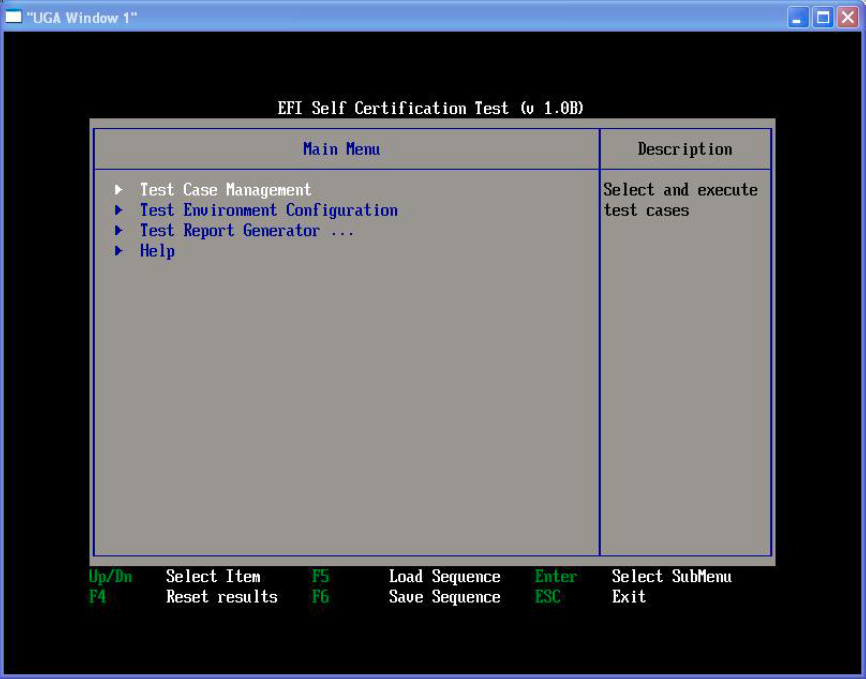
\includegraphics[height=8cm]{chart3/Main-Menu-Screen-Using-the-Menu-Driven-Interface}
			\caption{SCT的主界面菜单}
			\label{fig:Main-Menu-Screen-Using-the-Menu-Driven-Interface}
		\end{figure}
		
		主界面分为四个部分:
		
		\begin{itemize}
			\item 用例管理部分:用于在菜单中选择需要运行的用例,从而选择性的运行所需的用例。
			\item 测试环境的设置部分:通过修改测试环境的配置信息来控制其设置。
			\item 测试报告生成部分:用户利用其可以产生CSV格式的报告,并且存放到自动化测试工具主目录的Report目录中方便用户查看。
			\item 帮助信息部分。
		\end{itemize}
		
		此外在自动化测试工具的界面下可以使用快捷键方便用户操作,如表~\ref{tab:自动化测试工具SCT主界面的快捷键}所示:
		
		\begin{table}[H]
			\centering
			\caption{自动化测试工具SCT主界面的快捷键}
			\label{tab:自动化测试工具SCT主界面的快捷键}
			\begin{center}
			\begin{tabular}{|l|l|p{10cm}|} 
			\hline
			快捷键 & 功能 & 功能描述 \\ \hline
			F4 & 重置结果 & 重置所有的测试结果 \\ \hline
			F5 & 导入序列 & 从储存设备中导入测试序列文件,这一功能允许用户导入、编辑和执行现有的测试序列文件 \\ \hline
			F6 & 导出序列 & 将用户指定需要执行的用例的序列保存到一个文件 \\ \hline
			F8 & 继续执行 & 继续执行进行中剩余未执行的用例 \\ \hline
			F9 & 执行 & 执行测试工具识别到的所有用例 \\ \hline
			\end{tabular}
			\end{center}
		\end{table}
\begin{itemize}
	\item SCT的测试环境管理
		
		SCT的测试环境管理如图~\ref{fig:Test-Environment-Configuration}所示:	
		
		\begin{figure}[htbp] % use float package if you want it here
			\centering
			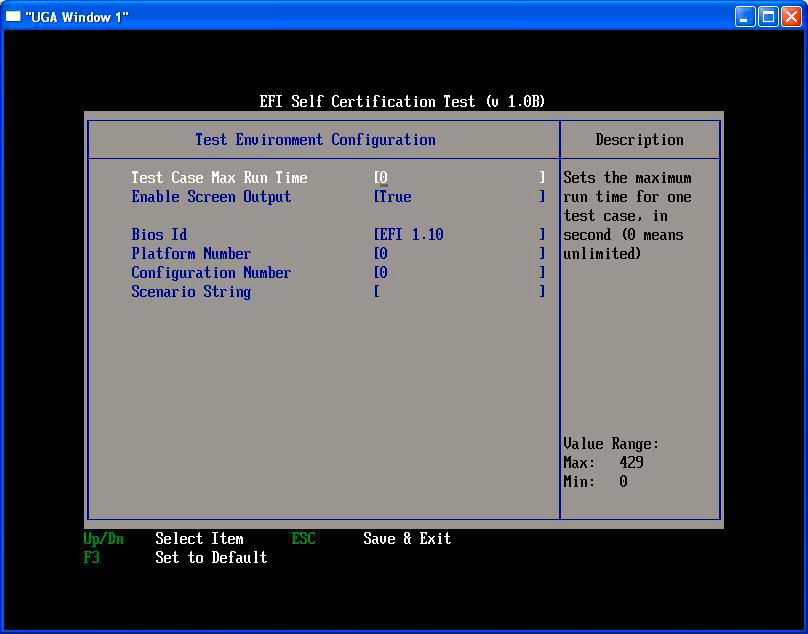
\includegraphics[height=8cm]{chart3/Test-Environment-Configuration}
			\caption{测试环境配置界面}
			\label{fig:Test-Environment-Configuration}
		\end{figure}
		
	\item SCT的用例管理
	
		SCT的用例配置管理界面主要是用来对用例进行控制和管理,如图~\ref{fig:Test-Case-Management-Screen}、~\ref{fig:Run-Time-Services-Screen}、~\ref{fig:使用seq测试序列文件来管理所需执行的测试用例}所示:
		
		\begin{figure}[H] % use float package if you want it here
			\centering
			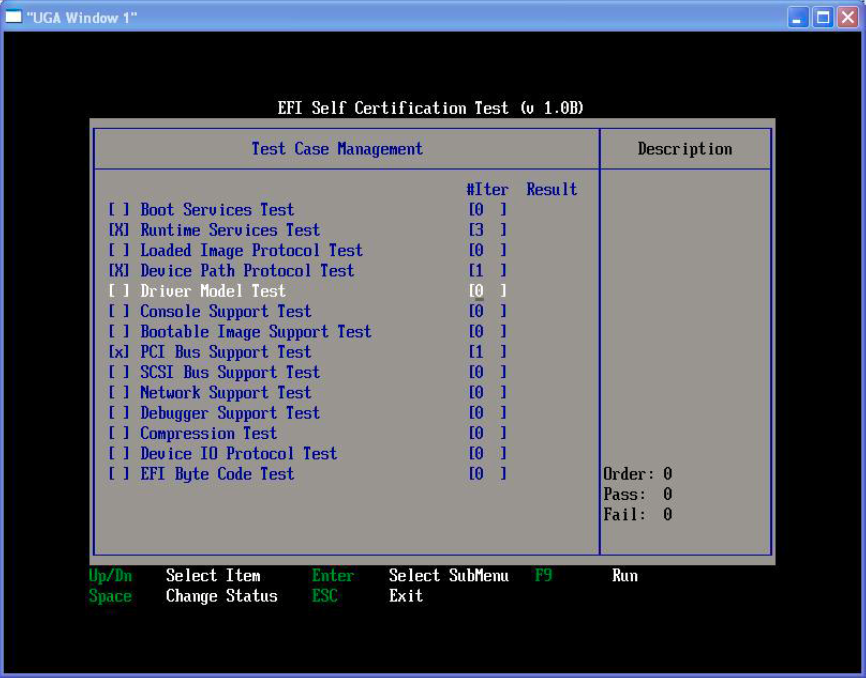
\includegraphics[height=8cm]{chart3/Test-Case-Management-Screen}
			\caption{用例管理界面}
			\label{fig:Test-Case-Management-Screen}
		\end{figure}
		
		\begin{figure}[H] % use float package if you want it here
			\centering
			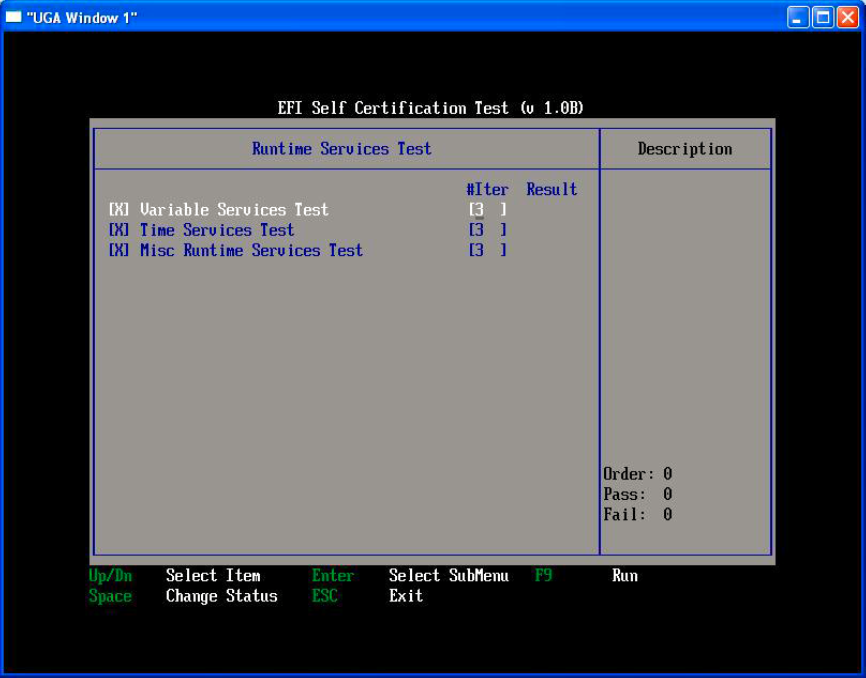
\includegraphics[height=8cm]{chart3/Run-Time-Services-Screen}
			\caption{用例执行次数管理界面}
			\label{fig:Run-Time-Services-Screen}
		\end{figure}
		
		\begin{figure}[H] % use float package if you want it here
			\centering
			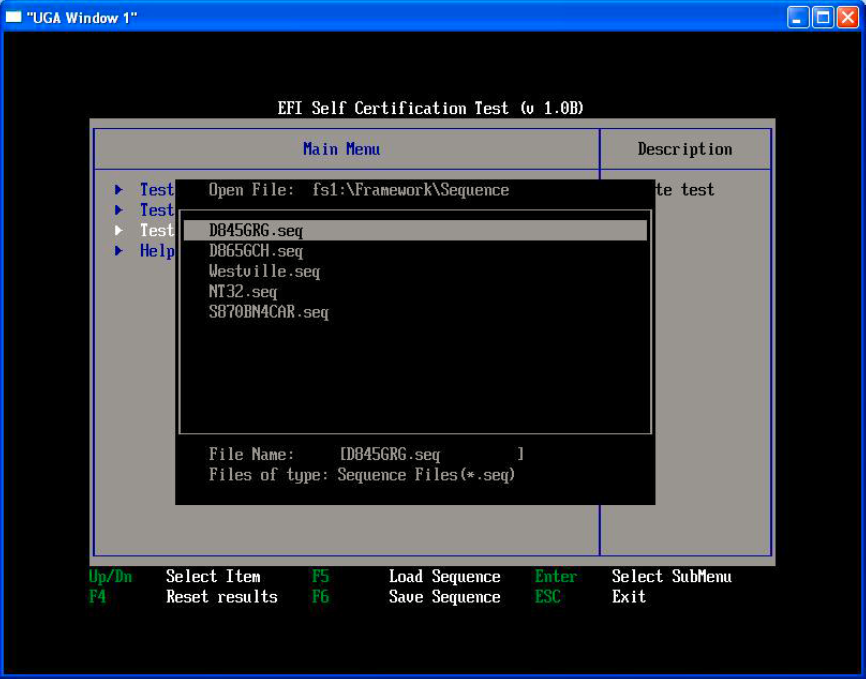
\includegraphics[height=8cm]{chart3/使用seq测试序列文件来管理所需执行的测试用例}
			\caption{使用seq测试序列文件来管理所需执行的测试用例}
			\label{fig:使用seq测试序列文件来管理所需执行的测试用例}
		\end{figure}
	
	\item SCT的测试报告生成器
	
		SCT的测试报告生成器主要用于对已执行完的日志和结果进行分析和总结,生成相应的测试报告。如图~\ref{fig:生成csv格式的测试报告}所示:
	
		\begin{figure}[H] % use float package if you want it here
			\centering
			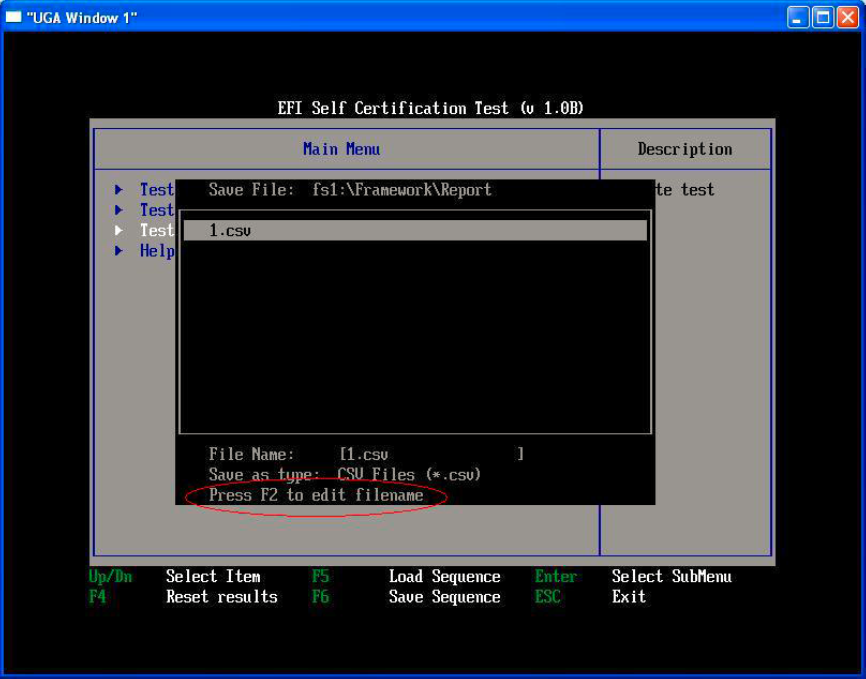
\includegraphics[height=8cm]{chart3/生成csv格式的测试报告}
			\caption{生成csv格式的测试报告}
			\label{fig:生成csv格式的测试报告}
		\end{figure}
		
\end{itemize}	
		
	\subsection{自动化测试工具的测试日志与报告}
	
		每一个用例在执行时,会自动将测试的进展情况写入到相应的日志文件中并且储存到测试工具主目录下对应的子目录中。每一个测试点都会相应对测试的结果进行记录,即Pass或者Failure。日志文件分为.log和.ekl两种不同类型的格式。.log日志文件是可读的文件,.ekl是供报告生成器分析的日志文件,两者仅在格式上有所区别。在所有的用例执行完成后,测试工具自带的报告生成器会解析其所有的.ekl文件,依据测试结果进行归类统计生成最后的CSV格式报表。CSV格式的文件在都有相应的软件可以打开,QA只需查看CSV中的信息便可了解此轮UEFI BIOS测试的结果。如图~\ref{fig:测试日志}、~\ref{fig:csv格式的测试报告可以使用Excel进行访问}所示:
		
		\begin{figure}[H] % use float package if you want it here
			\centering
			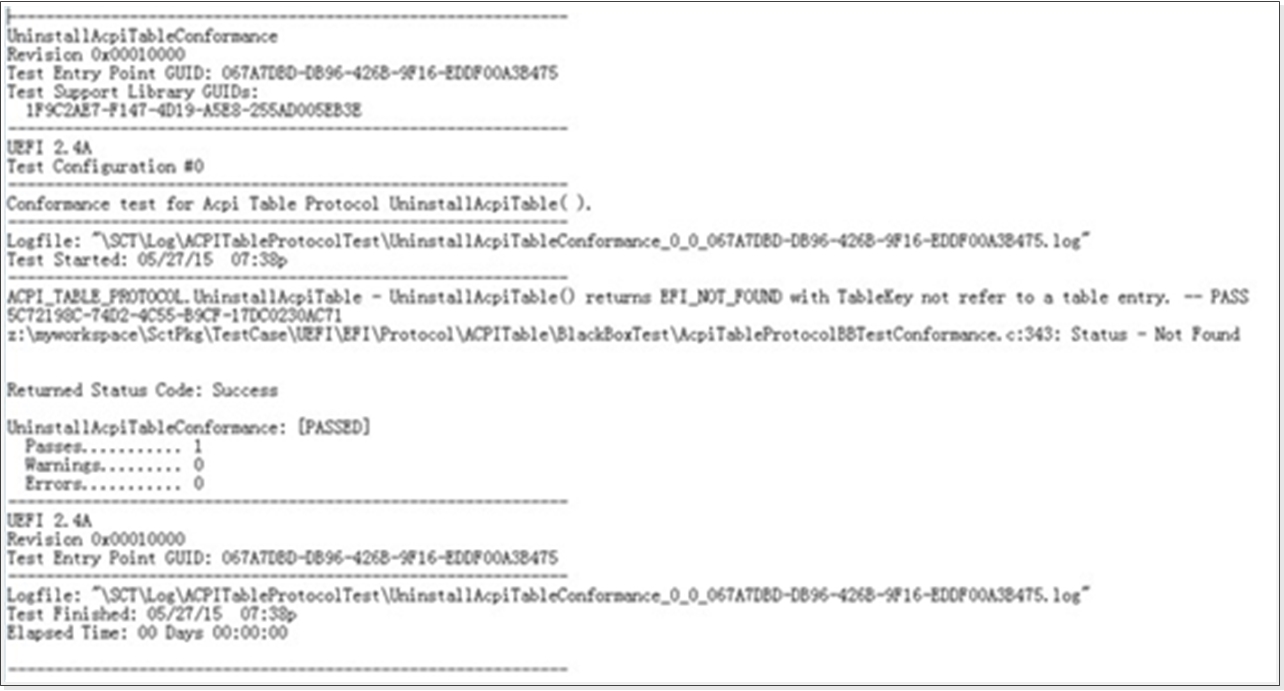
\includegraphics[height=7.5cm]{chart3/测试日志}
			\caption{测试日志}
			\label{fig:测试日志}
		\end{figure}
		
		\begin{figure}[H] % use float package if you want it here
			\centering
			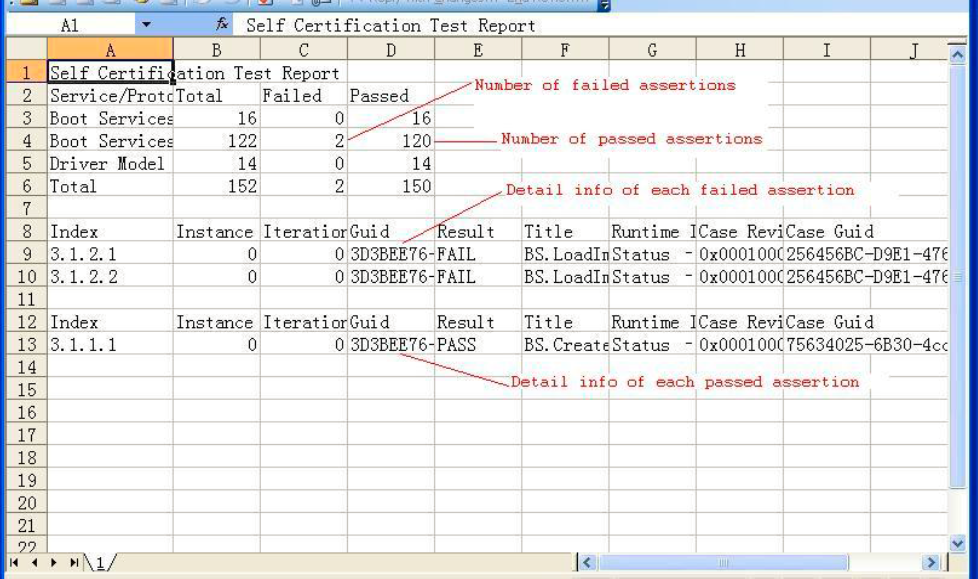
\includegraphics[height=8cm]{chart3/csv格式的测试报告可以使用Excel进行访问}
			\caption{csv格式的测试报告可以使用Excel进行访问}
			\label{fig:csv格式的测试报告可以使用Excel进行访问}
		\end{figure}
	
\section{本章小结}
   	
	本章主要分析了UEFI BIOS持续集成测试系统中所需的测试工具SCT的设计,并且对其进行了实现。通过明确SCT的设计目标、对其进行需求分析,初步得出了其系统功能组成和系统功能流程,并且进一步对其进行具体设计与实现,最后讲述该自动化测试工具的使用方法,以便于后续UEFI BIOS持续集成测试系统中对该工具的使用。
	
	目前SCT已成功实现并且通过验证,应用于UEFI BIOS的测试工作,即便是没有代码经验的QA也能方便、快捷、高质量的使用其完成对UEFI BIOS产品质量的自动化测试工作,在产品的不断迭代与更新中起到了非常重要的效果和应用价值。

	